%!TEX root = *.tex
%%%%%%%%%%%%%%%%%%
% カウンタのリセット
\setcounter{figure}{0}
% 問題文

図1のように,直流電源$\text{E}_1$,抵抗$\text{R}_1$,抵抗$\text{R}_2$,コンデンサー$\text{C}_1$,コンデンサー$\text{C}_2$,スイッチ$\text{S}_1$で構成された回路を考える.
$\text{E}_1$の起電力は$E$,
$\text{R}_1$と$\text{R}_2$の電気抵抗の値はともに$R$,
$\text{C}_1$と$\text{C}_2$の電気容量の値はともに$C$であり,
抵抗$\text{R}_1$と$\text{R}_2$以外の電気抵抗の値は無視できるものとする.
全てのコンデンサーの初期電荷は$0$である.
また,時刻$t<0$では,スイッチ$\text{S}_1$は開いている.

まず,スイッチ$\text{S}_1$を$\text{A}_1$に接続した場合を考える.
$\text{C}_1$の極板間の電圧の大きさを$V_0$とし,
図のように抵抗$\text{R}_1$に上向きに流れる電流を$I_1$とする.
なお,接続したときの時刻を$t=0$とする.
以下の設問に答えよ.





\begin{enumerate}[(1)]
  \setlength{\leftskip}{-1zw}
  \setlength{\itemindent}{1zw}\setlength{\labelsep}{0.5zw}
  \setlength{\labelwidth}{1zw}\setlength{\leftmargin}{1zw}
  \setlength{\itemsep}{0.5\baselineskip}
  \item スイッチ$\text{S}_1$を$\text{A}_1$に接続した直後における電流$I_1$を$E,\,C,\,R$のうち必要なものを用いて表せ.
  \item $t>0$において,電流$I_1$の時間変化を表すグラフの概形として最も適切なものを以下の選択肢より一つ選べ.
\end{enumerate}

\noindent 選択肢:\par 
\begin{figure}[H]
  \centering
  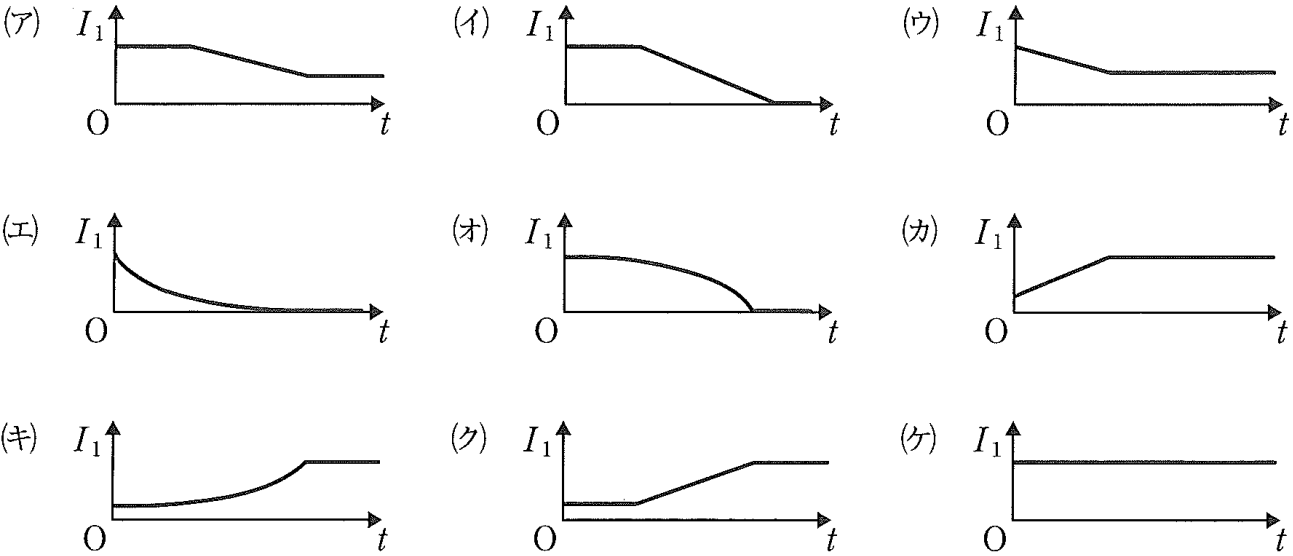
\includegraphics[width=.8\columnwidth]{../graphs/nagoya_23_2-2.png}
\end{figure}

\begin{enumerate}[(1)]
  \setlength{\leftskip}{-1zw}
  \setlength{\itemindent}{1zw}\setlength{\labelsep}{0.5zw}
  \setlength{\labelwidth}{1zw}\setlength{\leftmargin}{1zw}
  \setlength{\itemsep}{0.5\baselineskip}
  \addtocounter{enumi}{2}
  \item 十分に時間が経過したときの$V_0$を$E,\,C,\,R$のうち必要なものを用いて表せ.
\end{enumerate}

スイッチ$\text{S}_1$を$\text{A}_1$に接続した状態で十分に時間が経過したのち,
スイッチ$\text{S}_1$を$\text{B}_1$に切り換える.
以下の設問に答えよ.

\begin{enumerate}[(1)]
  \setlength{\leftskip}{-1zw}
  \setlength{\itemindent}{1zw}\setlength{\labelsep}{0.5zw}
  \setlength{\labelwidth}{1zw}\setlength{\leftmargin}{1zw}
  \setlength{\itemsep}{0.5\baselineskip}
  \addtocounter{enumi}{3}
  \item スイッチ$\text{S}_1$を$\text{B}_1$に切り換え,十分に時間が経過したときの$V_0$を$E,\,C,\,R$のうち必要なものを用いて表せ.
  \item スイッチ$\text{S}_1$を$\text{B}_1$に切り換えたのち,十分に時間が経過するまでに$\text{R}_2$で消費されるエネルギーを$E,\,C,\,R$のうち必要なものを用いて表せ.
\end{enumerate}



図2は,図1の回路の抵抗$\text{R}_2$をコイル$\text{L}_1$に置き替えた回路である.
$\text{L}_1$の自己インダクタンスの値は$L$であり,抵抗$\text{R}_1$以外の電気抵抗は無視できるものとする.
全てのコンデンサーの初期電荷は$0$である.

この回路では,スイッチ$\text{S}_1$を$\text{A}_1$に接続して十分に時間が経過したのち,
$\text{S}_1$を$\text{B}_1$に切り換えたところ,電気振動が起きた.
以下の設問に答えよ.

\begin{enumerate}[(1)]
  \setlength{\leftskip}{-1zw}
  \setlength{\itemindent}{1zw}\setlength{\labelsep}{0.5zw}
  \setlength{\labelwidth}{1zw}\setlength{\leftmargin}{1zw}
  \setlength{\itemsep}{0.5\baselineskip}
  \addtocounter{enumi}{5}
  \item $\text{C}_2$に蓄えられる電荷の最大値を$E,\,C,\,L$のうち必要なものを用いて表せ.
  \item $\text{L}_1$に流れる電流の絶対値が最大値$I_{\rm m}$になったとき,コイル$\text{L}_1$の両端の電圧は0である.
  $E=1.00\,\text{V},\,C=0.100\,\text{mF},\,L=5.00\,\text{mH}$のとき$I_{\rm m}$の値を有効数字2桁で求めよ.
  なお,$1\,\text{mF}=10^{-3}\,\text{F},\,1\,\text{mH}=10^{-3}\,\text{H}$である.
\end{enumerate}

\begin{comment}

{
\begin{wrapfigure}{r}{.3\columnwidth}
  \vspace{-\intextsep}
  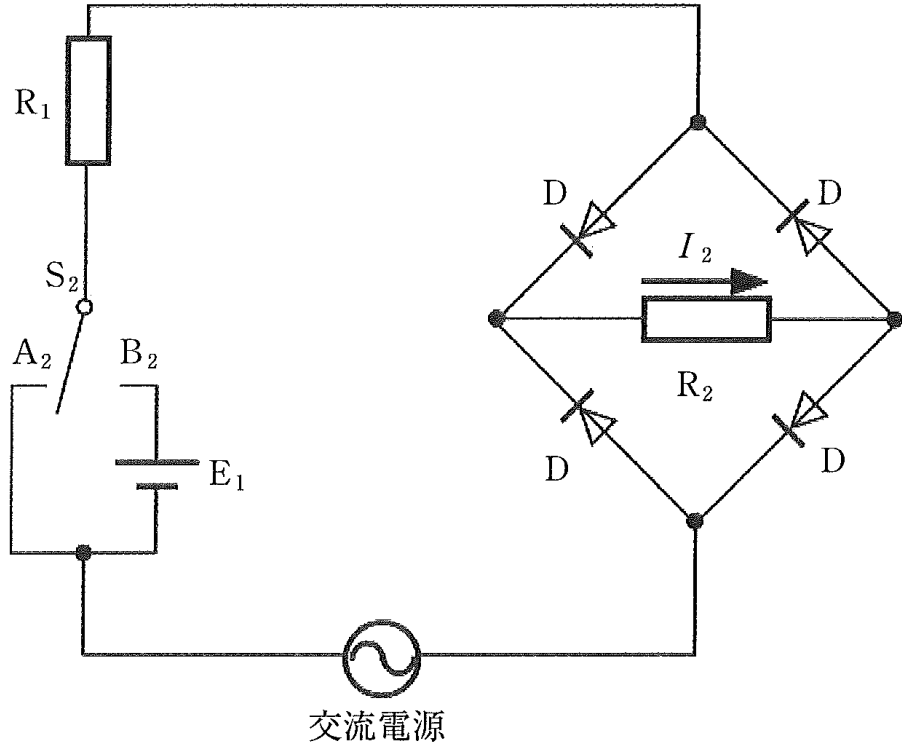
\includegraphics[width=.3\columnwidth]{../graphs/nagoya_23_2-4.png}
\end{wrapfigure}

図3のように直流電源$\text{E}_1$,正弦波交流の電源,抵抗$\text{R}_1$,抵抗$\text{R}_2$,Dで示すダイオード4つ,スイッチ$\text{S}_2$を接続した回路を考える.
$\text{E}_1$の起電力は$E$,正弦波交流電源の電圧の振幅は$2E$,
$\text{R}_1$と$\text{R}_2$の電気抵抗の値はともに$R$であり,
抵抗$\text{R}_1$と$\text{R}_2$以外の電気抵抗の値は無視できるものとする.
4つのダイオードは全て同じものであり,
整流作用のみを持つ理想化された素子として考える.
図のように抵抗$\text{R}_2$を右向きに流れる電流を$I_2$とする.
以下の設問に答えよ.

\par}

\begin{enumerate}[(1)]
  \setlength{\leftskip}{-1zw}
  \setlength{\itemindent}{1zw}\setlength{\labelsep}{0.5zw}
  \setlength{\labelwidth}{1zw}\setlength{\leftmargin}{1zw}
  \setlength{\itemsep}{0.5\baselineskip}
  \addtocounter{enumi}{7}
  \item スイッチ$\text{S}_2$を$\text{A}_2$に接続したとき,および$\text{B}_2$に接続したときを考える.$\text{R}_2$に流れる電流$I_2$の時間変化を表すグラフの概形として最も適切なものを以下の選択肢より一つ選べ.
\end{enumerate}

\noindent 選択肢:\par 
\begin{figure}[H]
  \centering
  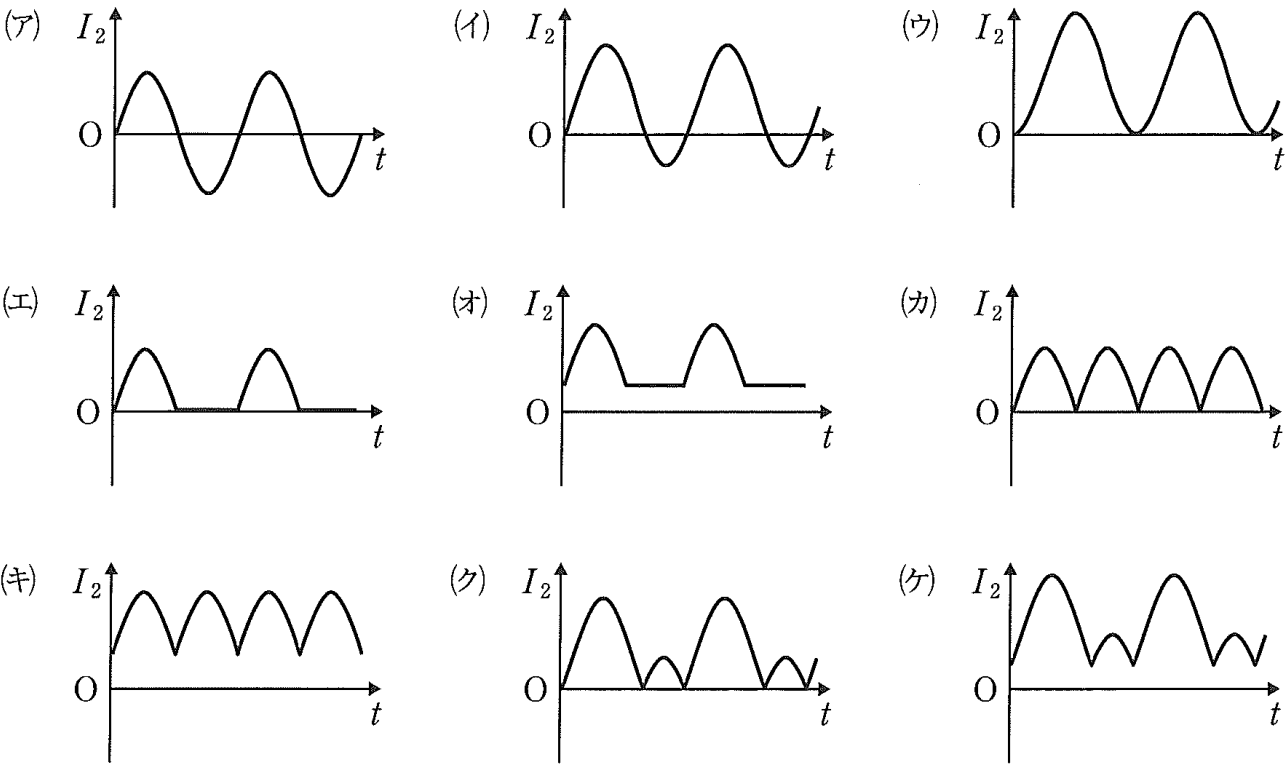
\includegraphics[width=.8\columnwidth]{../graphs/nagoya_23_2-5.png}
\end{figure}

\end{comment}


\begin{figure}[H]
  \centering
  \begin{minipage}{.4\columnwidth}
    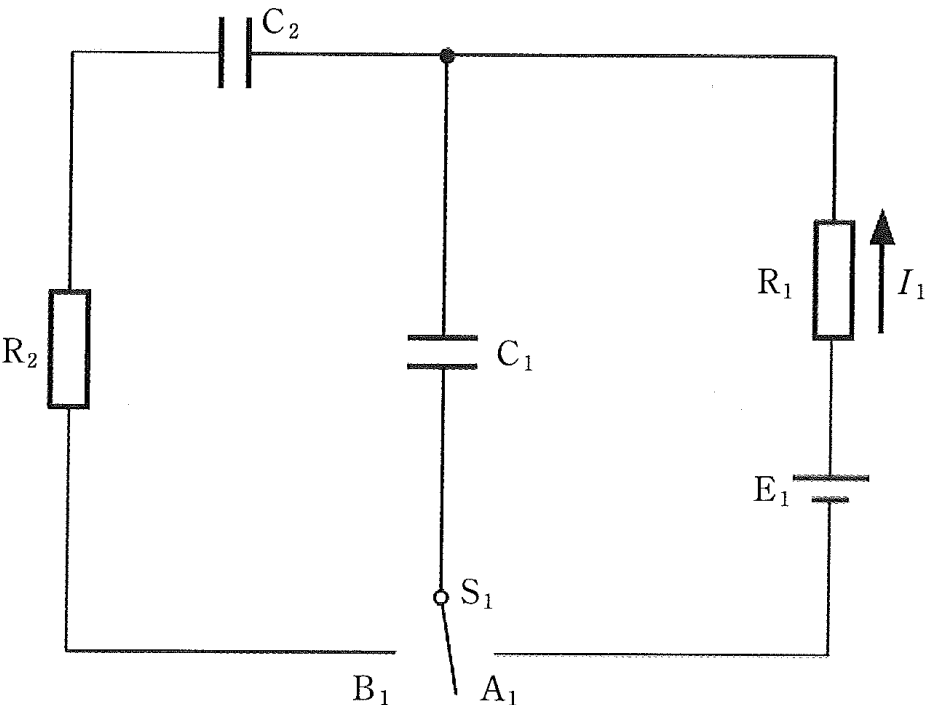
\includegraphics[width=\columnwidth]{../graphs/nagoya_23_2-1.png}
    \caption{}
  \end{minipage}
  \hspace{.1\columnwidth}
  \begin{minipage}{.4\columnwidth}
    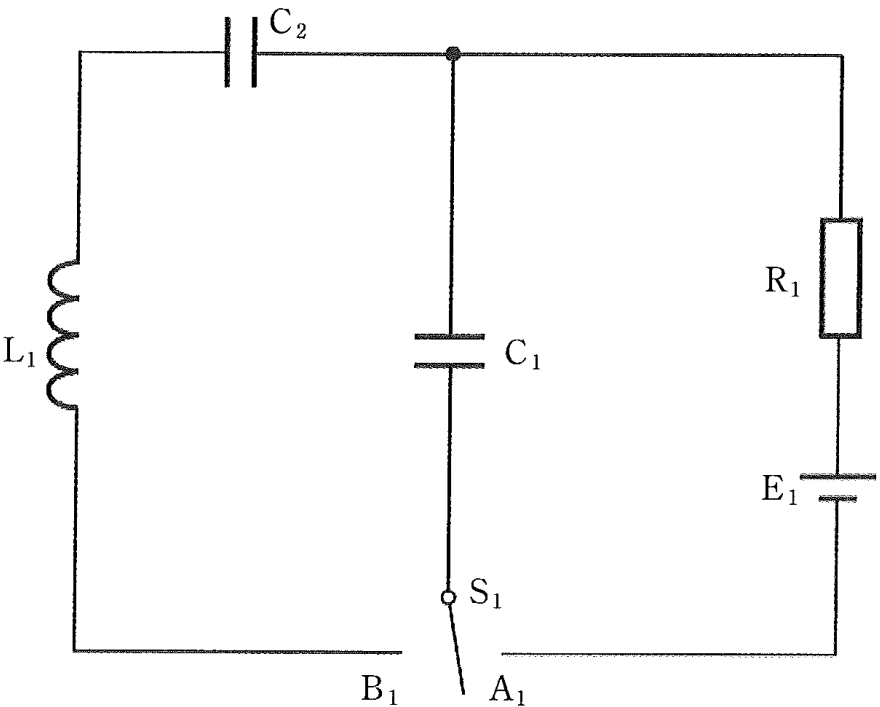
\includegraphics[width=\columnwidth]{../graphs/nagoya_23_2-3.png}
    \caption{} 
  \end{minipage}
\end{figure}


% メモ
\begin{comment}

\end{comment}


%%%%%%%%%%%%%%%%%%
